
%(BEGIN_QUESTION)
% Copyright 2012, Tony R. Kuphaldt, released under the Creative Commons Attribution License (v 1.0)
% This means you may do almost anything with this work of mine, so long as you give me proper credit

Interpret the temperature measurement displayed by this gauge mechanism, and also identify the meaning of the {\it other} pointer:

$$\epsfxsize=6in 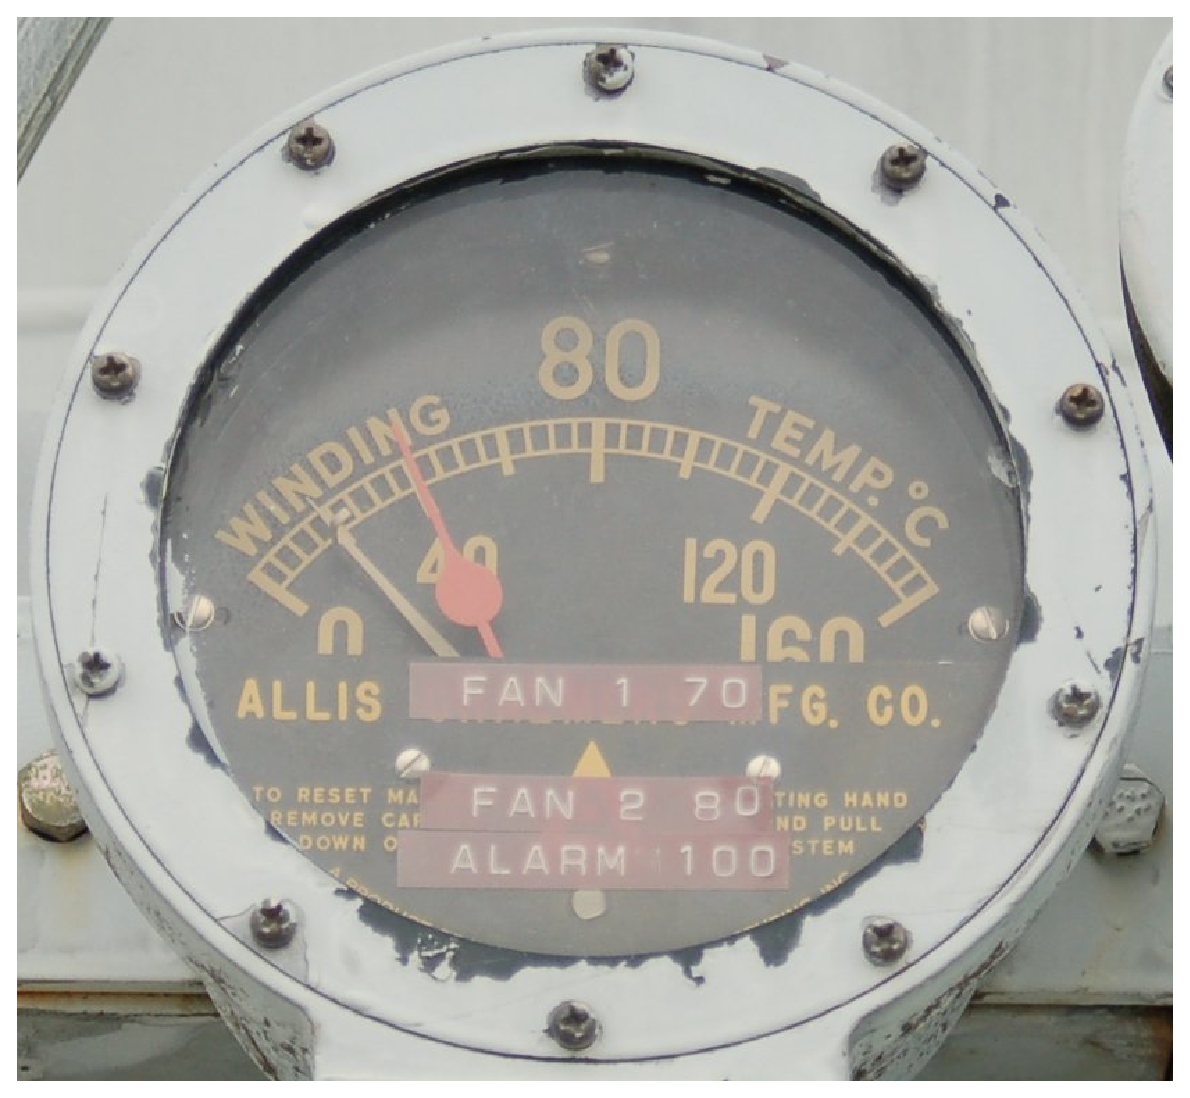
\includegraphics[width=15.5cm]{i02063x01.eps}$$

\underbar{file i02063}
%(END_QUESTION)





%(BEGIN_ANSWER)

The current temperature is 40 degrees Celsius (red pointer), and the other pointer is a low-temperature capture.  In this case, the ``capture'' pointer shows that the temperature went down as low as 20 degrees Celsius (or perhaps a bit lower, since parallax error is making that pointer appear to read higher than it actually is).
 
%(END_ANSWER)





%(BEGIN_NOTES)


%INDEX% Measurement, analog gauge reading

%(END_NOTES)


